
\subsection{Baseline}

We implement a classification-based baseline inspired by the Raidar method \cite{mao2024raidargenerativeaidetection}, which detects machine-generated content via rewriting. The key idea is that large language models (LLMs) tend to make fewer edits when rewriting content originally generated by another LLM, as opposed to human-written text, which they tend to revise more extensively. This concept can be further extended to hypothesize that an LLM will make even fewer edits when rewriting text originally generated by itself, compared to text generated by a different LLM. This is due to the structural and stylistic consistencies within the outputs of a given LLM, which make its own generations more "acceptable" or lower-loss candidates during rewriting. As a result, measuring the degree of rewriting not only helps distinguish AI-generated from human text, but also allows us to infer the specific model that likely generated the input.

As illustrated in Figure~\ref{fig:baseline_pipeline}, our method prompts a fixed rewriting model (e.g., GPT-3.5-Turbo) with a standardized instruction (e.g., “Concise this for me and keep all the information”) to rewrite the input text. The figure visually demonstrates that human-written inputs typically result in larger modifications during rewriting—highlighted by numerous character-level insertions and deletions—whereas AI-generated inputs lead to much smaller changes, reflecting the model's tendency to preserve its own generative style.

In our classification-based baseline, for each input text, we prompt multiple candidate LLMs (e.g., GPT variants) to rewrite the text and compute the edit distance between their rewritten output and the original input using the Levenshtein metric. The model whose rewrite is closest (i.e., has the minimum edit distance) is predicted as the most likely generator of the input. If all edit distances exceed a predefined threshold—chosen as the \textbf{median} of the \textbf{maximum edit distance} across training samples—the input is classified as human-written. 

\begin{center}
    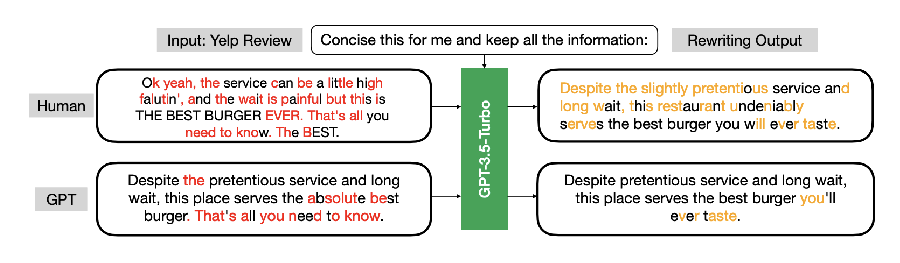
\includegraphics[width=0.9\textwidth]{image/raidar_image.pdf}
    \captionof{figure}{\textbf{Illustration of Raidar concept.} Given a Yelp review, GPT-3.5-Turbo is asked to rewrite the input text while preserving meaning. The rewriting of a human-written review undergoes more character-level edits (highlighted in red/orange), while the rewriting of a GPT-written review remains largely unchanged.}
    \label{fig:baseline_pipeline}
\end{center}
